% begin module EVT-statement
\begin{frame}[t]
\begin{theorem}[The Extreme Value Theorem]
If $f$ is continuous on a closed interval $[a,b]$, then $f$ attains its absolute maximum value $f(c)$ and its absolute minimum value $f(d)$ at some numbers $c$ and $d$ in $[a,b]$.
\end{theorem}
\begin{columns}[c]
\column{.3\textwidth}
\ \uncover<2->{%
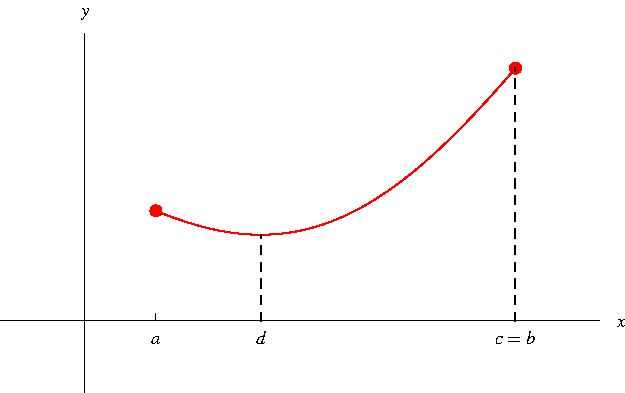
\includegraphics[width=4cm]{maxima-minima/pictures/04-01-evtb.pdf}%
}%
\column{.3\textwidth}
\ 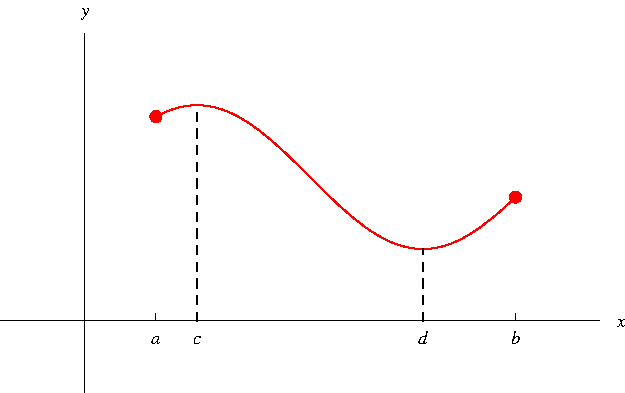
\includegraphics[width=4cm]{maxima-minima/pictures/04-01-evta.pdf}%
\column{.3\textwidth}
\ \uncover<3->{%
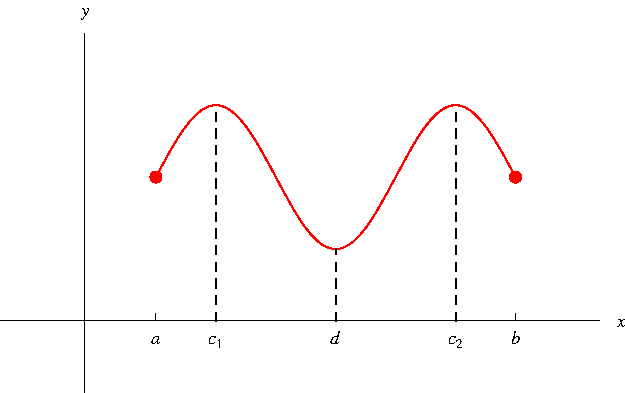
\includegraphics[width=4cm]{maxima-minima/pictures/04-01-evtc.pdf}%
}%
\end{columns}
\begin{itemize}
\item<2-| alert@2>  Extreme values might happen at endpoints.
\item<3-| alert@3>  Extreme values might happen twice.
\end{itemize}
\end{frame}
% end module EVT-statement
